%----------------------------------
% Evaluation of CID Section
%----------------------------------
\section{Evaluation of CID}

% Slide: Evaluation of CID Introduction
\begin{frame}
  \frametitle{Evaluation of CID}
  \begin{itemize}
    \item \textbf{Research Questions}
    \begin{itemize}
      \item \textbf{RQ4}: How accurate is CID in detecting incorrect responses?
      \item \textbf{RQ5}: How do the base and mutation challenge prompts impact performance?
    \end{itemize}
  \end{itemize}
\end{frame}

% Slide: Benchmark Study Setup
\begin{frame}
  \frametitle{Benchmark Study Setup}
  \begin{itemize}
    \item \textbf{Context}: Software Library Selection Task
    \item \textbf{Dataset Collection}:
    \begin{itemize}
      \item Collected 100 Stack Overflow (SO) posts
      \item Focused on text processing libraries: \textbf{spaCy}, \textbf{NLTK}, \textbf{GSON}
      \item Covered aspects like ease of use, performance, stability, etc.
    \end{itemize}
    \item \textbf{Base Questions}:
    \begin{itemize}
      \item Formulated questions based on SO posts
      \item Example: \textit{"How easy is it to use the library strictly based on the following conversation?"}
    \end{itemize}
  \end{itemize}
\end{frame}

% Slide: Visualizing the Benchmark Setup
\begin{frame}
  \frametitle{Visualizing the Benchmark Setup}
  \begin{center}
    \begin{tikzpicture}[node distance=2cm, auto, thick, scale=0.7, transform shape]
      % Define styles for active and inactive nodes
      \tikzstyle{activeblock} = [rectangle, draw, fill=blue!20, text width=3cm, text centered, rounded corners, minimum height=1cm, opacity=1]
      \tikzstyle{inactiveblock} = [rectangle, draw, fill=blue!20, text width=3cm, text centered, rounded corners, minimum height=1cm, opacity=0.3]
      \tikzstyle{activeline} = [draw, -latex', opacity=1]
      \tikzstyle{inactiveline} = [draw, -latex', opacity=0.3]
      
      % Nodes
      \node<1-4> [activeblock] (posts) {Stack Overflow Posts};
      \node<1> [inactiveblock, right of=posts, node distance=4cm] (extract) {Extract Q\&A Pairs};
      \node<1> [inactiveblock, right of=extract, node distance=4cm] (questions) {Formulate Base Questions};
      \node<1> [inactiveblock, right of=questions, node distance=4cm] (chatgpt) {Obtain ChatGPT Responses};

      \node<2-4> [activeblock, right of=posts, node distance=4cm] (extract) {Extract Q\&A Pairs};
      \node<2> [inactiveblock, right of=extract, node distance=4cm] (questions) {Formulate Base Questions};
      \node<2> [inactiveblock, right of=questions, node distance=4cm] (chatgpt) {Obtain ChatGPT Responses};

      \node<3-4> [activeblock, right of=extract, node distance=4cm] (questions) {Formulate Base Questions};
      \node<3> [inactiveblock, right of=questions, node distance=4cm] (chatgpt) {Obtain ChatGPT Responses};

      \node<4> [activeblock, right of=questions, node distance=4cm] (chatgpt) {Obtain ChatGPT Responses};

      % Arrows
      \path<1> [inactiveline] (posts) -- (extract);
      \path<2-4> [activeline] (posts) -- (extract);
      
      \path<1-2> [inactiveline] (extract) -- (questions);
      \path<3-4> [activeline] (extract) -- (questions);
      
      \path<1-3> [inactiveline] (questions) -- (chatgpt);
      \path<4> [activeline] (questions) -- (chatgpt);
    \end{tikzpicture}
    \captionof{figure}{Flowchart of Benchmark Study Setup}
  \end{center}
\end{frame}



% Slide: CID Components Diagram
\begin{frame}
  \frametitle{CID Components Recap}

    % Items at the top for each overlay
      \only<1>{
      \textbf{ENQUIRER}
      \begin{itemize}
        \item Extracts explanations from ChatGPT's base responses
      \end{itemize}
      }
      \only<2>{
      \textbf{CHALLENGER} 
      \begin{itemize}
        \item Poses basic and mutated challenge questions
        \item Uses metamorphic relationships to mutate questions
      \end{itemize}
      }
      \only<3>{\textbf{DECIDER}
      \begin{itemize}
        \item Analyzes inconsistencies
        \item Employs ML techniques to detect incorrectness
      \end{itemize}
      }
  
    \vspace{0.5cm} % Add some space between items and diagram

  \begin{center}
    \begin{tikzpicture}[node distance=3cm, auto, thick, scale=0.6, transform shape]
      % Define styles for active and inactive nodes
      \tikzstyle{activeblock} = [rectangle, draw, fill=blue!20, text width=2.8cm, text centered, rounded corners, minimum height=1cm, opacity=1]
      \tikzstyle{inactiveblock} = [rectangle, draw, fill=blue!20, text width=2.8cm, text centered, rounded corners, minimum height=1cm, opacity=0.3]
      \tikzstyle{activeline} = [draw, -latex', opacity=1]
      \tikzstyle{inactiveline} = [draw, -latex', opacity=0.3]

      % Nodes and Arrows with Overlays
      % Overlay 1: Highlight Enquirer
      \only<1>{
        \node [activeblock] (enquirer) {Enquirer};
        \node [inactiveblock, right=of enquirer, xshift=1cm] (challenger) {Challenger};
        \node [inactiveblock, right=of challenger, xshift=1cm] (decider) {Decider};

        \path [inactiveline] (enquirer) -- node [above, yshift=0.2cm] {Explanations} (challenger);
        \path [inactiveline] (challenger) -- node [above, yshift=0.2cm] {Challenge Responses} (decider);
        \draw [inactiveline] (decider.south) |- ++(0,-1.5cm) -| node [below, pos=0.5, yshift=-0.2cm, xshift=7.1cm] {Feedback} (enquirer.south);
      }

      % Overlay 2: Highlight Enquirer and Challenger
      \only<2>{
        \node [activeblock] (enquirer) {Enquirer};
        \node [activeblock, right=of enquirer, xshift=1cm] (challenger) {Challenger};
        \node [inactiveblock, right=of challenger, xshift=1cm] (decider) {Decider};

        \path [activeline] (enquirer) -- node [above, yshift=0.2cm] {Explanations} (challenger);
        \path [inactiveline] (challenger) -- node [above, yshift=0.2cm] {Challenge Responses} (decider);
        \draw [inactiveline] (decider.south) |- ++(0,-1.5cm) -| node [below, pos=0.5, yshift=-0.2cm, xshift=7.1cm] {Feedback} (enquirer.south);
      }

      % Overlay 3: Highlight all components
      \only<3>{
        \node [activeblock] (enquirer) {Enquirer};
        \node [activeblock, right=of enquirer, xshift=1cm] (challenger) {Challenger};
        \node [activeblock, right=of challenger, xshift=1cm] (decider) {Decider};

        \path [activeline] (enquirer) -- node [above, yshift=0.2cm] {Explanations} (challenger);
        \path [activeline] (challenger) -- node [above, yshift=0.2cm] {Challenge Responses} (decider);
        \draw [activeline] (decider.south) |- ++(0,-1.5cm) -| node [below, pos=0.5, yshift=-0.2cm, xshift=7.1cm] {Feedback} (enquirer.south);
      }

    \end{tikzpicture}
    \captionof{figure}{Interaction between CID Components}
  \end{center}
\end{frame}




% Slide: Explanation Generation (Text)
\begin{frame}
  \frametitle{Explanation Generation}
    \textbf{Process}:
    \begin{itemize}
      \item ChatGPT provides base responses to base questions
      \item ENQUIRER requests separate explanations for each piece of information
    \end{itemize}
\end{frame}

% Slide: Explanation Generation (Figure)
\begin{frame}
  \frametitle{Explanation Generation}
  \vspace{0.5cm}
  \textbf{Outcome}:
    \begin{itemize}
      \item Generated 341 explanations from 100 posts
      \item \textbf{Labeling}:
      \begin{itemize}
        \item \only<1>{\textbf{\textcolor{mygreen}{276 explanations (81\%) labeled as correct}}}
              \only<2>{\textcolor{mygreen!20}{276 explanations (81\%) labeled as correct}}
        \item \only<2>{\textbf{\textcolor{myred}{65 explanations (19\%) labeled as incorrect}}}
              \only<1>{\textcolor{myred!20}{65 explanations (19\%) labeled as incorrect}}
      \end{itemize}
    \end{itemize}
  \begin{center}
    \begin{tikzpicture}[scale=0.5, transform shape]
      % First overlay: Highlight Correct Explanations
      \only<1>{
        \pie[
          color = {mygreen!70, myred!15},
          explode = {0.1, 0},
          text = legend,
          sum = 100,
        ]{81/Correct Explanations, 19/Incorrect Explanations}
      }
      % Second overlay: Highlight Incorrect Explanations
      \only<2>{
        \pie[
          color = {mygreen!15, myred!70},
          explode = {0, 0.1},
          text = legend,
          sum = 100,
        ]{81/Correct Explanations, 19/Incorrect Explanations}
      }
    \end{tikzpicture}
    \captionof{figure}{Distribution of Correct and Incorrect Explanations}
  \end{center}
\end{frame}






% Slide: Incorrectness Detection Performance (RQ4) (Text)
\begin{frame}
  \frametitle{Incorrectness Detection Performance (RQ4)}
  \begin{itemize}
    \item \textbf{Machine Learning Models Evaluated}:
    \begin{itemize}
      \item Logistic Regression (LR)
      \item Random Forest (RF)
      \item Support Vector Machine (SVM)
    \end{itemize}
    \item \textbf{Performance Metrics}:
    \begin{itemize}
      \item Precision (P), Recall (R), F1-Score (F1), Accuracy (A)
    \end{itemize}
  \end{itemize}
  % \vspace{0.2cm}
  \begin{center}
    \small
    \begin{tabular}{lrrrr}
    \toprule
     \textbf{Model} & \textbf{P} & \textbf{R} & \textbf{A} & \textbf{F1} \\ \midrule
    Logistic Regression (LR) & 0.74 & 0.65 & 0.65 & 0.68 \\ 
    Random Forest (RF) & 0.73 & 0.65 & 0.65 & 0.68 \\ 
    Support Vector Machine (SVM) & \textbf{0.74} & \textbf{0.75} & \textbf{0.75} & \textbf{0.74} \\ 
    \bottomrule
    \end{tabular}
    \captionof{table}{ML model performance to detect ChatGPT incorrectness}
    \label{tab:model_accuracy}
  \end{center}
\end{frame}


% Slide: Visualizing Model Performance
\begin{frame}
  \frametitle{Visualizing Model Performance}
  \begin{center}
    \begin{tikzpicture}[scale=0.8,transform shape]
    \begin{axis}[
      ybar,
      bar width=15pt, % Increased bar width
      width=10cm,
      height=6cm,
      enlarge x limits=0.2,
      legend style={
        at={(0.5,-0.25)},
        anchor=north,
        legend columns=2
      },
      symbolic x coords={LR, RF, SVM},
      xtick={LR, RF, SVM}, % Explicitly set x-axis ticks
      xticklabels={Logistic Regression (LR), Random Forest (RF), Support Vector Machine (SVM)},
      x tick label style={
        text width=3cm,
        align=center,
        font=\small,
      },
      ylabel={Metric Value},
      ymin=0.6, ymax=0.8,
      nodes near coords,
      nodes near coords align={vertical},
      every node near coord/.append style={font=\scriptsize}, % Smaller font size
    ]


  
        % Data for Accuracy (Blue Bars)
        \addplot+[
          draw=blue, fill=blue!70,
          bar shift=-12pt, % Increased spacing between red and blue bars
          opacity=1, % Fully opaque for highlighted bar
          visible on=<1>
        ] coordinates {(LR,0.65)};
        \addplot+[
          draw=blue, fill=blue!70,
          bar shift=-12pt,
          opacity=0.3, % Less opaque for non-highlighted bars
          visible on=<1>
        ] coordinates {(RF,0.65)};
        \addplot+[
          draw=blue, fill=blue!70,
          bar shift=-12pt,
          opacity=0.3,
          visible on=<1>
        ] coordinates {(SVM,0.75)};
  
        % Highlight RF on Slide 2
        \addplot+[
          draw=blue, fill=blue!70,
          bar shift=-12pt,
          opacity=0.3,
          visible on=<2>
        ] coordinates {(LR,0.65)};
        \addplot+[
          draw=blue, fill=blue!70,
          bar shift=-12pt,
          opacity=1,
          visible on=<2>
        ] coordinates {(RF,0.65)};
        \addplot+[
          draw=blue, fill=blue!70,
          bar shift=-12pt,
          opacity=0.3,
          visible on=<2>
        ] coordinates {(SVM,0.75)};
  
        % Highlight SVM on Slide 3
        \addplot+[
          draw=blue, fill=blue!70,
          bar shift=-12pt,
          opacity=0.3,
          visible on=<3>
        ] coordinates {(LR,0.65)};
        \addplot+[
          draw=blue, fill=blue!70,
          bar shift=-12pt,
          opacity=0.3,
          visible on=<3>
        ] coordinates {(RF,0.65)};
        \addplot+[
          draw=blue, fill=blue!70,
          bar shift=-12pt,
          opacity=1,
          visible on=<3>
        ] coordinates {(SVM,0.75)};
  
        % Data for F1-Score (Red Bars)
        \addplot+[
          draw=red, fill=red!70,
          bar shift=12pt, % Increased spacing between red and blue bars
          opacity=1,
          visible on=<1>
        ] coordinates {(LR,0.68)};
        \addplot+[
          draw=red, fill=red!70,
          bar shift=12pt,
          opacity=0.3,
          visible on=<1>
        ] coordinates {(RF,0.68)};
        \addplot+[
          draw=red, fill=red!70,
          bar shift=12pt,
          opacity=0.3,
          visible on=<1>
        ] coordinates {(SVM,0.74)};
  
        % Highlight RF on Slide 2
        \addplot+[
          draw=red, fill=red!70,
          bar shift=12pt,
          opacity=0.3,
          visible on=<2>
        ] coordinates {(LR,0.68)};
        \addplot+[
          draw=red, fill=red!70,
          bar shift=12pt,
          opacity=1,
          visible on=<2>
        ] coordinates {(RF,0.68)};
        \addplot+[
          draw=red, fill=red!70,
          bar shift=12pt,
          opacity=0.3,
          visible on=<2>
        ] coordinates {(SVM,0.74)};
  
        % Highlight SVM on Slide 3
        \addplot+[
          draw=red, fill=red!70,
          bar shift=12pt,
          opacity=0.3,
          visible on=<3>
        ] coordinates {(LR,0.68)};
        \addplot+[
          draw=red, fill=red!70,
          bar shift=12pt,
          opacity=0.3,
          visible on=<3>
        ] coordinates {(RF,0.68)};
        \addplot+[
          draw=red, fill=red!70,
          bar shift=12pt,
          opacity=1,
          visible on=<3>
        ] coordinates {(SVM,0.74)};
  
        % Legends for Metrics (Appears on Slide 3)
        \only<3>{
          \addlegendimage{draw=blue,fill=blue!70}
          \addlegendentry{Accuracy}
          \addlegendimage{draw=red,fill=red!70}
          \addlegendentry{F1-Score}
          \legend{}
        }
  
      \end{axis}
    \end{tikzpicture}
    \captionof{figure}{Comparison of ML Model Performances}
  \end{center}
\end{frame}

% Slide: Misclassification Analysis (Donut Chart)
\begin{frame}
  \frametitle{Misclassification Analysis}

  \begin{itemize}
    \item \textbf{Total Misclassifications}: 86 out of 341 explanations
  \end{itemize}

  \only<2-5>{\begin{itemize}
    \item \textbf{Error Sources} (44\% of errors)
    \begin{itemize}
      \only<2>{\item 
        \textbf{Decider Component} (44\% of errors)
        \begin{itemize}
          \item Similarity calculation issues
          \item Difficulty detecting unanimous incorrect responses
        \end{itemize}
      }
      \only<3>{\item 
        \textbf{Challenger Component} (32\% of errors)
        \begin{itemize}
          \item Misdirected challenges
          \item Out-of-scope questions
        \end{itemize}
      }
      \only<4>{\item 
        \textbf{Enquirer Component} (5\% of errors)
        \begin{itemize}
          \item Convoluted explanations with multiple opinions
        \end{itemize}
      }
      \only<5>{\item 
        \textbf{Mixed Sources} (19\% of errors)
        \begin{itemize}
          \item Continuous incorrect reasoning by ChatGPT
          \item Generic issues (unclear information)
        \end{itemize}
      }
    \end{itemize}
  \end{itemize}}
  

  \centering % Center the content
  \vspace{0.5cm}
  \begin{center}
  % Define colors within the frame
  \begin{tikzpicture}[scale=0.5, transform shape]
    % Local color definitions
    \definecolor{DeciderColor}{RGB}{102, 102, 238}    % Blue
    \definecolor{ChallengerColor}{RGB}{119, 209, 243}  % Green
    \definecolor{EnqColor}{RGB}{241, 230, 145}        % Orange
    \definecolor{MixedColor}{RGB}{244, 182, 114}     % Purple
    \definecolor{GreyColor}{RGB}{192, 192, 192}     % Grey for blurred slices

    % Overlay 1: Highlight Decider
    \only<1>{
        \pie[
      cloud,
      text=inside,
      scale font,
      radius=3, % Increased radius for more space
      % Optionally adjust font size
      color={
          DeciderColor,
          ChallengerColor,
          EnqColor,
          MixedColor
        },
      font=\scriptsize
    ]{
      44/Decider,
      32/Challenger,
      5/Enq., % Abbreviated label
      19/Mixed
    }
    }
    \only<2>{
      \pie[
        cloud,
        text=inside,
        scale font,
        radius=3,
        color={
          DeciderColor,
          GreyColor,
          GreyColor,
          GreyColor
        },
        font=\scriptsize
      ]{
        44/Decider,
        32/Challenger,
        5/Enq.,
        19/Mixed
      }
    }

    % Overlay 2: Highlight Challenger
    \only<3>{
      \pie[
        cloud,
        text=inside,
        scale font,
        radius=3,
        color={
          GreyColor,
          ChallengerColor,
          GreyColor,
          GreyColor
        },
        font=\scriptsize
      ]{
        44/Decider,
        32/Challenger,
        5/Enq.,
        19/Mixed
      }
    }

    % Overlay 3: Highlight Enquirer
    \only<4>{
      \pie[
        cloud,
        text=inside,
        scale font,
        radius=3,
        color={
          GreyColor,
          GreyColor,
          EnqColor,
          GreyColor
        },
        font=\scriptsize
      ]{
        44/Decider,
        32/Challenger,
        5/Enq.,
        19/Mixed
      }
    }

    % Overlay 4: Highlight Mixed
    \only<5>{
      \pie[
        cloud,
        text=inside,
        scale font,
        radius=3,
        color={
          GreyColor,
          GreyColor,
          GreyColor,
          MixedColor
        },
        font=\scriptsize
      ]{
        44/Decider,
        32/Challenger,
        5/Enq.,
        19/Mixed
      }
    }
  \end{tikzpicture}
\end{center}

  % Caption below the chart
  \captionof{figure}{Distribution of Error Sources}

\end{frame}


% Slide: Impact of Challenge Prompts (RQ5) (Text)
% Slide: Impact of Challenge Prompts (Merged)
\begin{frame}
  \frametitle{Impact of Challenge Prompts (RQ5)}

  % Slide 1: Experiment Setup

    \begin{itemize}
      \item \textbf{Experiment Setup}:
      \begin{itemize}
        \item Evaluated the impact of individual challenge prompts
        \item Tested performance by excluding each question type
      \end{itemize}
    \end{itemize}


  % Slide 2: Table of Results
    \begin{center}
      \small
      \begin{tabular}{lrr}
      \toprule
      \textbf{Scenarios} & \textbf{Accuracy} & \textbf{F1-score} \\ \midrule
      With all questions & 0.75 & 0.74 \\
      Without \textit{How} questions & 0.75 & 0.75 \\
      Without \textit{Really} questions & 0.69 & 0.70 \\ 
      Without \textit{Why} questions & 0.70 & 0.71 \\ 
      \bottomrule         
      \end{tabular}
      \captionof{table}{Impact of individual challenge prompts}
      \label{tab:challenge_question_impact}
    \end{center}
\end{frame}


% Slide: Visualizing Impact of Challenge Prompts
\begin{frame}
  \frametitle{Visualizing Impact of Challenge Prompts}
  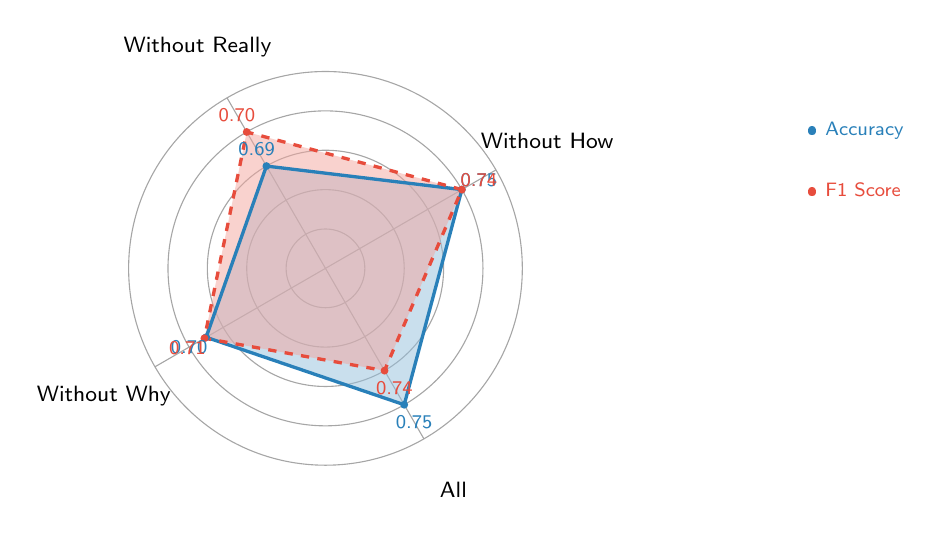
\begin{tikzpicture}[scale=0.5]
      % Color definitions
      \definecolor{accuracycolor}{RGB}{41, 128, 185}
      \definecolor{f1color}{RGB}{231, 76, 60}
      
      % Radar chart parameters
      \def\maxradius{5}
      
      % Draw background grid
      \foreach \r in {1,2,3,4,5} {
          \draw[gray!70] (0,0) circle (\r);
      }
      
      % Draw axes
      \foreach \angle/\label in {
          30/Without How, 
          120/Without Really, 
          210/Without Why, 
          300/All
      } {
          \draw[gray!70] (\angle:\maxradius) -- (\angle:0);
          \node[font=\footnotesize\sffamily] at (\angle:\maxradius+1.5) {\label};
      }
      
      % Accuracy values (scaled by 5)
      \def\accuracyWithoutHow{4}
      \def\accuracyWithoutReally{3}
      \def\accuracyWithoutWhy{3.5}
      \def\accuracyAll{4}
      
      % F1 Score values (scaled by 5)
      \def\FWithoutHow{4}
      \def\FWithoutReally{4}
      \def\FWithoutWhy{3.55}
      \def\FAll{3}
      
      % Accuracy polygon
      \fill[
          accuracycolor!50,
          opacity=0.5
      ] 
          (30:\accuracyWithoutHow) -- 
          (120:\accuracyWithoutReally) -- 
          (210:\accuracyWithoutWhy) -- 
          (300:\accuracyAll) -- cycle;
      
      % F1 Score polygon
      \fill[
          f1color!50,
          opacity=0.5
      ] 
          (30:\FWithoutHow) -- 
          (120:\FWithoutReally) -- 
          (210:\FWithoutWhy) -- 
          (300:\FAll) -- cycle;
      
      % Accuracy outline
      \draw[
          accuracycolor,
          very thick
      ] 
          (30:\accuracyWithoutHow) -- 
          (120:\accuracyWithoutReally) -- 
          (210:\accuracyWithoutWhy) -- 
          (300:\accuracyAll) -- cycle;
      
      % F1 Score outline
      \draw[
          f1color,
          very thick,
          dashed
      ] 
          (30:\FWithoutHow) -- 
          (120:\FWithoutReally) -- 
          (210:\FWithoutWhy) -- 
          (300:\FAll) -- cycle;
      
      % Value markers for Accuracy
      \foreach \angle/\value in {
          30/\accuracyWithoutHow, 
          120/\accuracyWithoutReally, 
          210/\accuracyWithoutWhy, 
          300/\accuracyAll
      } {
          \fill[accuracycolor] (\angle:\value) circle (0.1);
      }
      
      % Value markers for F1 Score
      \foreach \angle/\value in {
          30/\FWithoutHow, 
          120/\FWithoutReally, 
          210/\FWithoutWhy, 
          300/\FAll
      } {
          \fill[f1color] (\angle:\value) circle (0.1);
      }
      
      % Value labels for Accuracy
      \foreach \angle/\value/\display in {
          30/\accuracyWithoutHow/0.75, 
          120/\accuracyWithoutReally/0.69, 
          210/\accuracyWithoutWhy/0.70, 
          300/\accuracyAll/0.75
      } {
          \node[font=\scriptsize\sffamily, text=accuracycolor] at (\angle:{\value + 0.5}) {\display};
      }
      
      % Value labels for F1 Score
      \foreach \angle/\value/\display in {
          30/\FWithoutHow/0.74, 
          120/\FWithoutReally/0.70, 
          210/\FWithoutWhy/0.71, 
          300/\FAll/0.74
      } {
          \node[font=\scriptsize\sffamily, text=f1color] at (\angle:{\value + 0.5}) {\display};
      }
      
      % Legend
      % Original positions: (6,3) and (6,2.5)
      % Adjusted positions to add more space
      \node[font=\scriptsize\sffamily, text=accuracycolor, anchor=west] at (12,3.5) {\textbf{•} Accuracy};
      \node[font=\scriptsize\sffamily, text=f1color, anchor=west] at (12,2) {\textbf{•} F1 Score};

  \end{tikzpicture}
  \end{frame}

% Slide: Impact of Mutation and Basic Challenges
\begin{frame}
  \frametitle{Impact of Mutation \& Basic Challenges}

  % Slide 1: Key Findings
    \begin{itemize}
      \item \textbf{Key Findings}:
      \begin{itemize}
        \item Excluding mutation challenges reduced accuracy by 16\% (from 75\% to 63\%)
        \item Excluding basic challenges reduced accuracy by 8\% (from 75\% to 69\%)
      \end{itemize}
    \end{itemize}

  % Slide 2: Table of Results
    \begin{center}
      \small
      \begin{tabular}{lrr}
      \toprule
      \textbf{Scenarios} & \textbf{Accuracy} & \textbf{F1-score} \\ \midrule
      With Basic and Mutation Challenges & 0.75 & 0.74 \\ 
      Without Mutation Challenges & 0.63 & 0.65 \\ 
      Without Basic Challenges & 0.69 & 0.69 \\ 
      \bottomrule
      \end{tabular}
      \captionof{table}{Impact of mutation \& basic challenges}
      \label{tab:mutation_impact}
    \end{center}
\end{frame}


% Slide: Visualizing Impact of Mutation & Basic Challenges
\begin{frame}
  \frametitle{Visualizing Impact of Mutation \& Basic Challenges}
  \begin{center}
    \begin{tikzpicture}[scale=0.9, transform shape]
      \begin{axis}[
        width=10cm,
        height=6cm,
        symbolic x coords={With Both, Without Mutation, Without Basic},
        xtick=data,
        xticklabels={}, % Remove x-axis labels
        ylabel={Performance Metric},
        ymin=0.60, ymax=0.80,
        legend style={
          at={(0.5,-0.15)},
          anchor=north,
          legend columns=-1
        },
        grid=major, % Optional: Adds a grid for better readability
      ]
      
        % -----------------------------
        % Overlay 1: Accuracy Prominent
        % F1-Score Blurred
        % -----------------------------
        \only<1>{
          % Accuracy Line: Blue with Square Markers (Full Opacity)
          \addplot[
            color=blue,
            mark=square*,
            line width=1.5pt,
          ]
          coordinates {
            (With Both,0.75)
            (Without Mutation,0.63)
            (Without Basic,0.69)
          };
          
          % F1-Score Line: Red with Circular Markers (Blurred)
          \addplot[
            color=red,
            mark=*,
            line width=1.5pt,
            opacity=0.2
          ]
          coordinates {
            (With Both,0.74)
            (Without Mutation,0.65)
            (Without Basic,0.69)
          };
        }
        
        % -----------------------------
        % Overlay 2: F1-Score Prominent
        % Accuracy Blurred
        % -----------------------------
        \only<2>{
          % Accuracy Line: Blue with Square Markers (Blurred)
          \addplot[
            color=blue,
            mark=square*,
            line width=1.5pt,
            opacity=0.2
          ]
          coordinates {
            (With Both,0.75)
            (Without Mutation,0.63)
            (Without Basic,0.69)
          };
          
          % F1-Score Line: Red with Circular Markers (Full Opacity)
          \addplot[
            color=red,
            mark=*,
            line width=1.5pt,
          ]
          coordinates {
            (With Both,0.74)
            (Without Mutation,0.65)
            (Without Basic,0.69)
          };
        }
        
        % -----------------------------
        % Legend (Consistent Across Overlays)
        % -----------------------------
        \only<1,2>{
          \legend{Accuracy, F1-Score}
        }
        
      \end{axis}
    \end{tikzpicture}
    \captionof{figure}{Impact of Mutation and Basic Challenges}
  \end{center}
\end{frame}


% Slide: Example of Mutation Impact (Text)
\begin{frame}
  \frametitle{Example of Mutation Impact}
  \begin{itemize}
    \item \textbf{Scenario}:
    \begin{itemize}
      \item Base Explanation: "The library's performance is great but complex to configure."
    \end{itemize}
  \end{itemize}
\end{frame}

% Animation: Mutation Impact (Step 1)
\begin{frame}
  \frametitle{Example of Mutation Impact - Basic Challenge}
  \begin{itemize}
    \item \textbf{Basic Challenge}:
    \begin{itemize}
      \item Question: "Why is the library complex to configure?"
      \item ChatGPT Response: Provides a general answer
    \end{itemize}
  \end{itemize}
  \begin{center}
    \begin{tikzpicture}[node distance=5cm, auto, thick, scale=0.8, transform shape]
      % Define styles for active and inactive nodes
      \tikzstyle{activeblock} = [rectangle, draw, text width=3.5cm, text centered, rounded corners, minimum height=1cm, font=\small, opacity=1]
      \tikzstyle{inactiveblock} = [rectangle, draw, text width=3.5cm, text centered, rounded corners, minimum height=1cm, font=\small, opacity=0.3]
      \tikzstyle{activeline} = [draw, -latex', opacity=1]
      \tikzstyle{inactiveline} = [draw, -latex', opacity=0.3]
    
      % Nodes
      \node<1-3> [activeblock, fill=blue!20] (base) {Base Explanation: \par "The library's performance is great but complex to configure."};
      \node<1> [inactiveblock, fill=green!20, right of=base] (basic) {Basic Challenge: \par "Why is the library complex to configure?"};
      \node<1> [inactiveblock, fill=yellow!20, right of=basic] (response) {ChatGPT Response: Provides a general answer};
      
      \node<2-3> [activeblock, fill=green!20, right of=base] (basic) {Basic Challenge: \par "Why is the library complex to configure?"};
      \node<2> [inactiveblock, fill=yellow!20, right of=basic] (response) {ChatGPT Response: Provides a general answer};
      
      \node<3> [activeblock, fill=yellow!20, right of=basic] (response) {ChatGPT Response: Provides a general answer};
    
      % Arrows
      \path<1> [inactiveline] (base) -- (basic);
      \path<2-3> [activeline] (base) -- (basic);
    
      \path<1-2> [inactiveline] (basic) -- (response);
      \path<3> [activeline] (basic) -- (response);
    \end{tikzpicture}
    
    
  \end{center}
\end{frame}

% Animation: Mutation Impact (Step 2)
\begin{frame}
  \frametitle{Example of Mutation Impact - Mutation Challenge}
  \begin{itemize}
    \item \textbf{Mutation Challenge}:
    \begin{itemize}
      \item Question: "Why is the library complex to configure, especially when integrating with legacy systems?"
      \item ChatGPT Response: Reveals inconsistencies or additional issues
    \end{itemize}
  \end{itemize}
  \begin{center}
    \begin{tikzpicture}[node distance=5cm, auto, thick, scale=0.6, transform shape]
      % Define styles for active and inactive nodes with different colors
      \tikzstyle{activeblock} = [rectangle, draw, text width=3cm, text centered, rounded corners, minimum height=1cm, font=\small, opacity=1]
      \tikzstyle{inactiveblock} = [rectangle, draw, text width=3cm, text centered, rounded corners, minimum height=1cm, font=\small, opacity=0.3]
      \tikzstyle{activeline} = [draw, -latex', opacity=1]
      \tikzstyle{inactiveline} = [draw, -latex', opacity=0.3]

      % Nodes with different colors for active states
      \node<1-4> [activeblock, fill=blue!30] (base) {Base Explanation: \par "The library's performance is great but complex to configure."};
      \node<1> [inactiveblock, fill=red!30, right of=base] (basic) {Basic Challenge: \par "Why is the library complex to configure?"};
      \node<1> [inactiveblock, fill=green!30, right of=basic] (mutation) {Mutation Challenge: \par "Why is the library complex to configure, especially when integrating with legacy systems?"};
      \node<1> [inactiveblock, fill=yellow!30, right of=mutation] (response) {ChatGPT Response: Reveals inconsistencies or additional issues};
      
      \node<2-4> [activeblock, fill=red!30, right of=base] (basic) {Basic Challenge: \par "Why is the library complex to configure?"};
      \node<2> [inactiveblock, fill=green!30, right of=basic] (mutation) {Mutation Challenge: \par "Why is the library complex to configure, especially when integrating with legacy systems?"};
      \node<2> [inactiveblock, fill=yellow!30, right of=mutation] (response) {ChatGPT Response: Reveals inconsistencies or additional issues};
      
      \node<3-4> [activeblock, fill=green!30, right of=basic] (mutation) {Mutation Challenge: \par "Why is the library complex to configure, especially when integrating with legacy systems?"};
      \node<3> [inactiveblock, fill=yellow!30, right of=mutation] (response) {ChatGPT Response: Reveals inconsistencies or additional issues};
      
      \node<4> [activeblock, fill=yellow!30, right of=mutation] (response) {ChatGPT Response: Reveals inconsistencies or additional issues};
      
      % Arrows
      \path<1> [inactiveline] (base) -- (basic);
      \path<2-4> [activeline] (base) -- (basic);
      
      \path<1-2> [inactiveline] (basic) -- (mutation);
      \path<3-4> [activeline] (basic) -- (mutation);
      
      \path<1-3> [inactiveline] (mutation) -- (response);
      \path<4> [activeline] (mutation) -- (response);
    \end{tikzpicture}
  \end{center}
\end{frame}


% Slide: Limitations Identified (Text)
\begin{frame}{Limitations of CID}
  \begin{itemize}
      \item \textbf{Dataset and Labeling Constraints}
      \begin{itemize}
          \item Relies on Stack Overflow data
          \item Variability and potential bias in human-annotated labels
      \end{itemize}
      
      \item \textbf{Similarity Measurement Challenges}
      \begin{itemize}
          \item Current metrics may struggle with complex or nuanced responses.
          \item Potential for misclassifications due to inadequate similarity assessments.
      \end{itemize}
      
      \item \textbf{Limited Scope and Generalizability}
      \begin{itemize}
          \item Evaluated primarily on software library selection tasks.
          \item Effectiveness on other SE tasks remains unexplored.
      \end{itemize}
  \end{itemize}
\end{frame}



% Slide: Summary of Evaluation (Text)
% \begin{frame}
%   \frametitle{Summary of Evaluation}
%   \begin{itemize}
%     \item \textbf{CID Performance}:
%     \begin{itemize}
%       \item Effectively detects incorrect responses
%       \item Mutation challenges are crucial for enhanced performance
%     \end{itemize}
%     \item \textbf{Implications}:
%     \begin{itemize}
%       \item Provides a tool for developers to assess ChatGPT's responses
%       \item Helps build trust and reliability in using AI assistants
%     \end{itemize}
%   \end{itemize}
%   \vspace{0.1cm}
%   \begin{center}
%   \begin{tikzpicture}[thick, scale=0.6, every node/.style={align=center}]
%     % Define styles for the nodes
%     \tikzstyle{block} = [circle, draw, text width=1.2cm, text centered, minimum height=1.2cm, font=\tiny, fill opacity=0.9]
    
%     % Nodes arranged on the circumference of a circle
%     \node [block, fill=blue!20] (perf) at (90:2cm) {CID\\Performance};
%     \node [block, fill=green!20] (mut) at (210:2cm) {Mutation\\Challenges};
%     \node [block, fill=yellow!20] (impl) at (330:2cm) {Implications};
    
%     % Curved arrows between nodes
%     \draw [->, thick, bend right=30] (perf) to (mut);
%     \draw [->, thick, bend right=30] (mut) to (impl);
%     \draw [->, thick, bend right=30] (impl) to (perf);
%   \end{tikzpicture}
%   \end{center}
% \end{frame}


%----------------------------------
% Conclusion Section
%----------------------------------
\section{Conclusion}

% Slide: Conclusion Overview
\begin{frame}
  \frametitle{Conclusion}
  \begin{itemize}
    \item \textbf{Recap of Research}:
    \begin{itemize}
     \only<1>{\item Explored developers' reliance on ChatGPT
      \item Identified concerns about response correctness}
      \only<2>{\item Developed CID to detect incorrect ChatGPT responses}
      \only<3>{\item Evaluted the performance of CID with relevant metrics}
    \end{itemize}
    \vspace{0.5cm}
    \begin{center}
    \begin{tikzpicture}[node distance=5cm, auto, thick, scale=0.7, transform shape]
      % Define styles for active and inactive nodes
      \tikzstyle{activeblock} = [rectangle, draw, text width=3cm, text centered, rounded corners, minimum height=1cm, font=\small, opacity=1]
      \tikzstyle{inactiveblock} = [rectangle, draw, text width=3cm, text centered, rounded corners, minimum height=1cm, font=\small, opacity=0.3]
      \tikzstyle{activeline} = [draw, -latex', opacity=1]
      \tikzstyle{inactiveline} = [draw, -latex', opacity=0.3]
    
      % Nodes
      \node<1-3> [activeblock, fill=blue!20] (survey) {Survey Insights};
      \node<1> [inactiveblock, fill=green!20, right of=survey] (cid) {CID Tool};
      \node<1> [inactiveblock, fill=yellow!20, right of=cid] (eval) {Evaluation Results};
    
      \node<2-3> [activeblock, fill=green!20, right of=survey] (cid) {CID Tool};
      \node<2> [inactiveblock, fill=yellow!20, right of=cid] (eval) {Evaluation Results};
    
      \node<3> [activeblock, fill=yellow!20, right of=cid] (eval) {Evaluation Results};
    
      % Arrows
      \path<1> [inactiveline] (survey) -- (cid);
      \path<2-3> [activeline] (survey) -- (cid);
    
      \path<1-2> [inactiveline] (cid) -- (eval);
      \path<3> [activeline] (cid) -- (eval);
    \end{tikzpicture}
  \end{center}
  \end{itemize}
\end{frame}


% Slide: Limitations
\begin{frame}
  \frametitle{Limitations}
  % \begin{itemize}
  %   \item \textbf{Dataset Dependence}
  %   \item \textbf{Similarity Measures}
  %   \item \textbf{Scope of Evaluation}
  % \end{itemize}
  \vspace{1cm}
  \begin{center}
    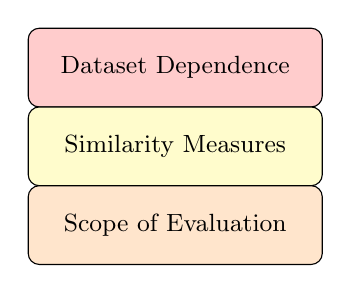
\begin{tikzpicture}
      \node [block, fill=red!20] (data) {Dataset Dependence};
      \node [block, fill=yellow!20, below of=data] (sim) {Similarity Measures};
      \node [block, fill=orange!20, below of=sim] (scope) {Scope of Evaluation};
    \end{tikzpicture}
    % \captionof{figure}{Summary of Limitations}
    
  \end{center}
  \begin{center}
  \vspace{0.5cm}
   \textbf{Summary of Limitations}
  \end{center}
\end{frame}

% Slide: Future Work
\begin{frame}
  \frametitle{Future Work}
  \begin{center}
    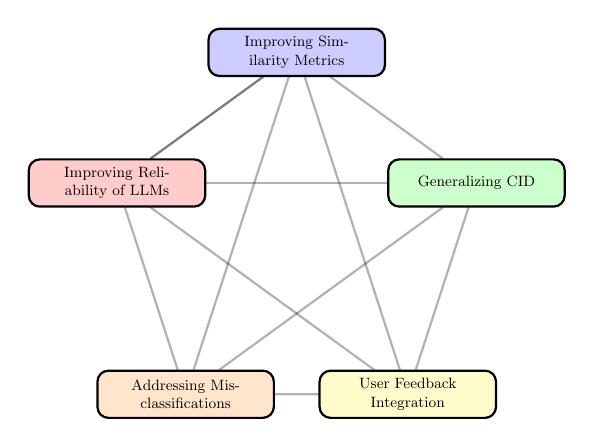
\begin{tikzpicture}[node distance=3cm, auto, thick, scale=0.6, transform shape]
      % Define node style
      \tikzstyle{block} = [rectangle, draw, rounded corners, text centered, text width=3.5cm, minimum height=1cm, font=\small]
    
      % Define pentagonal positions
      \node [block, fill=blue!20] (sim) at (90:4cm) {Improving Similarity Metrics};
      \node [block, fill=green!20] (gen) at (18:4cm) {Generalizing CID};
      \node [block, fill=yellow!20] (user) at (306:4cm) {User Feedback Integration};
      \node [block, fill=orange!20] (mis) at (234:4cm) {Addressing Misclassifications};
      \node [block, fill=red!20] (llm) at (162:4cm) {Improving Reliability of LLMs};
    
      % Undirected edges for full connectivity with reduced opacity
      \draw [-, thick, opacity=0.3] (sim) -- (gen);
      \draw [-, thick, opacity=0.3] (gen) -- (user);
      \draw [-, thick, opacity=0.3] (user) -- (mis);
      \draw [-, thick, opacity=0.3] (mis) -- (llm);
      \draw [-, thick, opacity=0.3] (llm) -- (sim);
    
      % Additional edges for full connectivity
      \draw [-, thick, opacity=0.3] (sim) -- (user);
      \draw [-, thick, opacity=0.3] (sim) -- (mis);
      \draw [-, thick, opacity=0.3] (sim) -- (llm);
    
      \draw [-, thick, opacity=0.3] (gen) -- (mis);
      \draw [-, thick, opacity=0.3] (gen) -- (llm);
    
      \draw [-, thick, opacity=0.3] (user) -- (llm);
    \end{tikzpicture}
    
    
    
    % \captionof{figure}{Future Work Roadmap}
    \vspace{0.5cm}
   \textbf{Future Work Roadmap}
  \end{center}
\end{frame}

\begin{frame}[allowframebreaks]
  \frametitle{References}
  
  \small
  \bibliographystyle{ACM-Reference-Format}
  
  \begin{thebibliography}{10}
  
  \bibitem{azaria2023internal}
  Amos Azaria and Tom Mitchell.
  \newblock The internal state of an {LLM} knows when it's lying.
  \newblock \emph{arXiv preprint arXiv:2304.13734}, 2023.
  
  \bibitem{jang2023consistency}
  Myeongjun Jang and Thomas Lukasiewicz.
  \newblock Consistency analysis of {ChatGPT}.
  \newblock \emph{arXiv preprint arXiv:2303.06273}, 2023.
  
  \bibitem{manakul2023selfcheckgpt}
  Potsawee Manakul, Adian Liusie, and Mark~J.~F. Gales.
  \newblock {SelfCheckGPT}: Zero-resource black-box hallucination detection for
    generative large language models.
  \newblock \emph{arXiv preprint arXiv:2303.08896}, 2023.
  
  \bibitem{feldman2023trapping}
  Philip Feldman, James~R. Foulds, and Shimei Pan.
  \newblock Trapping {LLM} hallucinations using tagged context prompts.
  \newblock \emph{arXiv preprint arXiv:2306.06085}, 2023.
  
  \bibitem{elazar2021measuring}
  Yanai Elazar, Nora Kassner, Shauli Ravfogel, Abhilasha Ravichander, Eduard
    Hovy, Hinrich Schütze, and Yoav Goldberg.
  \newblock Measuring and improving consistency in pretrained language models.
  \newblock \emph{Transactions of the Association for Computational Linguistics},
    9:1012--1031, 2021.
  
  \bibitem{larios2020selecting}
  Enrique Larios~Vargas, Maurício Aniche, Christoph Treude, Magiel Bruntink, and
    Georgios Gousios.
  \newblock Selecting third-party libraries: The practitioners' perspective.
  \newblock In \emph{Proceedings of the 28th ACM Joint Meeting on European
    Software Engineering Conference and Symposium on the Foundations of Software
    Engineering}, pages 245--256, 2020.
  
  \bibitem{uddin2017opiner}
  Gias Uddin and Foutse Khomh.
  \newblock {OPINER}: An opinion search and summarization engine for {APIs}.
  \newblock In \emph{Proceedings of the 32nd IEEE/ACM International Conference on
    Automated Software Engineering}, pages 978--983, 2017.
  
  \bibitem{uddin2019understanding}
  Gias Uddin, Olga Baysal, Latifa Guerrouj, and Foutse Khomh.
  \newblock Understanding how and why developers seek and analyze {API}-related
    opinions.
  \newblock \emph{IEEE Transactions on Software Engineering}, 47(4):694--735,
    2019.
  
  \bibitem{wang2020difftech}
  Han Wang, Chunyang Chen, Zhenchang Xing, and John Grundy.
  \newblock {DiffTech}: A tool for differencing similar technologies from
    question-and-answer discussions.
  \newblock In \emph{Proceedings of the 28th ACM Joint Meeting on European
    Software Engineering Conference and Symposium on the Foundations of Software
    Engineering}, pages 1576--1580, 2020.
  
  \bibitem{ribeiro2020beyond}
  Marco~Tulio Ribeiro, Tongshuang Wu, Carlos Guestrin, and Sameer Singh.
  \newblock Beyond accuracy: Behavioral testing of {NLP} models with {CheckList}.
  \newblock \emph{arXiv preprint arXiv:2005.04118}, 2020.

  \bibitem[Shen et~al\mbox{.}(2022)]%
        {shen2022natural}
  Qingchao Shen, Junjie Chen, Jie~M Zhang, Haoyu Wang, Shuang Liu, and Menghan Tian.
  \newblock Natural test generation for precise testing of question answering software. In {\emph{Proceedings of the 37th IEEE/ACM International Conference on Automated Software Engineering}}. pages 1--12.

  \vspace{0.5cm}
  \textbf{\Large Link to Orignal Paper\\}
  \href{https://dl.acm.org/doi/abs/10.1145/3597503.3639194}{ChatGPT Incorrectness Detection in Software Reviews}
  
  \end{thebibliography}
  
  \end{frame}

  

\setbeamercolor{background canvas}{bg=blue!20} % Set the background color globally for the slide
\begin{frame}
  \begin{center}
    \vspace{1cm} % Adjust vertical positioning
    {\Huge \textbf{\textit{Thank You!}}} % Large, aesthetic text
  \end{center}
\end{frame}






